\subsection{Results and discussion}

%%%%%%%%%%%%%%%%%%%%%%%%%%%%%%%%%%%%%%%%%%%%%%%%%%%%%%%%%%%%%%%%
%%  PocketVec performance on the ProSPECCTs benchmark sets  %%%%
%%%%%%%%%%%%%%%%%%%%%%%%%%%%%%%%%%%%%%%%%%%%%%%%%%%%%%%%%%%%%%%%

\phantomsection
\subsubsection{PocketVec performance on the ProSPECCTs benchmark sets}
\label{PocketVec_ResultsAndDiscussion_PocketVec_performance_on_the_ProSPECCTs_benchmark}

The performance of PocketVec descriptors across ProSPECCTs datasets is assessed in terms of the AUROC and is shown in Fig \ref{PocketVec_Fig1}d. We observe that PocketVec descriptors are robust to varying definitions of the same pocket, as determined by different crystallized ligands (P1, AUROC 0.97). When restricting such definitions to chemically similar ligands, the performance is maximal (P1.2, AUROC 1.00). Similarly, our descriptors are robust against protein conformational changes, i.e. protein flexibility (P2, AUROC 0.96), and they are also able to distinguish identical pockets from those altered by 5 artificial mutations leading to changes in physicochemical and shape properties of pocket-lining residues. In these cases, we obtained more modest performances (P3--physicochemical changes and P4--both physicochemical and shape changes, AUROCs of 0.67 and 0.72, respectively). Reassuringly though, we observed a significant correlation between the number of artificial mutations (1 to 5) and the corresponding AUROC values (Pearson CC > 0.98, p-value < 0.005 in both P3 and P4, Fig \ref{PocketVec_FigS9}), which confirmed that an increasing number of mutations in the binding site came along with an improved ability to detect such differences using PocketVec descriptors. 

We also benchmarked our descriptors in more biologically relevant scenarios where, for instance, pockets binding similar small molecules are found in structurally different proteins. ProSPECCTs includes two datasets to address such cases: P5 includes pocket structures classified into 9 distinct ligand classes (e.g. HEM, ATP, NAD, etc.), and P7 includes a realistic set of binding site pairs reported to be similar in published literature, some of them identified in otherwise unrelated proteins. In these sets, PocketVec descriptors show performances with AUROCs of 0.64 and 0.87, respectively, demonstrating their ability to identify similar pockets in globally dissimilar proteins. It is important to note that two binding sites having identical (or chemically similar) crystallized ligands are not necessarily similar from a PocketVec perspective. Following the logic behind the similarity ensemble approach (SEA\cite{keiser_relating_2007}), in which targets are quantitatively compared based on the chemical similarity of the ensemble of their ligands, a pair of targets sharing a single active compound may not be significantly similar.

Finally, with the goal of defining a PocketVec distance threshold to classify any pocket pair of interest as either similar or dissimilar, we analyzed the behavior of the Matthew's Correlation Coefficient (MCC) at multiple cut-off values across the different ProSPECCTs datasets (Fig \ref{PocketVec_FigS10}). As expected, each definition of pocket similarity in the ProSPECCTs datasets suggested the choice of a different cut-off distance. For instance, the optimal cut-off in the mutation-related benchmarks (P3 and P4) was around 0.13, while in the most realistic set of binding site pairs reported to be similar in published literature was even lower, around 0.08. However, for general purposes and to minimize false negatives, we selected the distance threshold based on the P1 dataset, where similar pairs were predefined as identical pockets binding chemically distinct ligands whereas dissimilar pairs were unrelated pockets binding different ligands. In this way, we defined 0.17 as our PocketVec threshold distance, which was the value maximizing the MCC in ProSPECCTs P1. However, this threshold should not be regarded as an absolute standard, but rather as a general guideline for classifying a pocket pair of interest as either similar or dissimilar.

For the sake of completeness, we generated results for all combinations of docking methods (rigid--rDock, and flexible--SMINA) and reduced sets of chemical compounds (128 LLM and 128 fragments). The use of rDock and LLM (128) was still the best strategy according to the ProSPECCTs datasets (Fig \ref{PocketVec_FigS11}). Besides, we observed that the selection of compounds leading to the most variable results throughout the different pockets (i.e. high entropy) was, indeed, of great help to distinguish similar from dissimilar pockets in ProSPECCTs P1. This effect was even more pronounced in the fragments, where their lower complexity and molecular weight led to higher promiscuity and redundancy (Fig \ref{PocketVec_FigS12}).

Detailed plots for all ProSPECCTs datasets including ROC Curves, PR Curves and distributions of PocketVec distances, docking scores and pocket volumes are included in our \hl{GitLab repository} (see \hyperref[PocketVec_Code]{Code and data availability}). 



%%%%%%%%%%%%%%%%%%%%%%%%%%%%%%%%%%%%%%%%%%%%%%%%%%%%%%%%%%%%%%%%
%%%%%%%%%%  Comparison with existing strategies  %%%%%%%%%%%%%%%
%%%%%%%%%%%%%%%%%%%%%%%%%%%%%%%%%%%%%%%%%%%%%%%%%%%%%%%%%%%%%%%%

\phantomsection
\subsubsection{Comparison with existing strategies}
\label{PocketVec_ResultsAndDiscussion_Comparison_with_existing_strategies}

Next, we compared the performance of PocketVec descriptors with state-of-the-art methodologies, as reported in several studies\cite{simonovsky_deeplytough_2020, scott_classification_2022, ehrt_benchmark_2018}, where the authors benchmarked many pocket comparison tools against the ProSPECCTs datasets, including six strategies based on pocket descriptors (Fig \ref{PocketVec_Fig1}d and Fig \ref{PocketVec_FigS11}). We used the AUROC as the standard performance measure to be able to compare our results with other available methodologies. However, for PocketVec descriptors, we also provide specific values of precision, accuracy, sensitivity, specificity, Matthew´s correlation coefficient and F1 score in each ProSPECCTs dataset (Fig \ref{PocketVec_FigS13}). Overall, PocketVec is the second-best ranked strategy in terms of the weighted average among datasets (0.89) and, indeed, it surpasses the median and the average performance in all ProSPECCTs datasets, apart from P3 (Table \ref{PocketVec_TableS1}). The top-scoring method is SiteAlign\cite{schalon_simple_2008}, which is alignment-dependent and based on the projection of residue descriptors into a triangle-discretized sphere that quantifies binding site similarity by minimizing distances between systematically generated cavity fingerprints obtained by moving one binding site with respect to the other. Thus, being specifically developed to compare pockets, it does not provide a unique descriptor for each binding site, which hampers the exploration of the pocket space in the same way molecular fingerprints do for the chemical space of small molecules. \hl{START} Other strategies are indeed alignment-free and provide unique representations for binding sites but, in addition to showing worse performances than PocketVec descriptors among ProSPECCTs datasets, also present several intrinsic limitations. For instance, KRIPO\cite{wood_pharmacophore_2012} and TIFP\cite{desaphy_encoding_2013} characterize protein-ligand binding interactions between receptors and bound ligands, which enables the identification of shared interaction patterns between pockets but limits their applicability domain to \textit{holo} structures. Additionally, FuzCav\cite{weill_alignment-free_2010} fingerprints count for specific pharmacophoric triplets of pocket-lining Cα, which enables the use of \textit{apo} structures but imply a simplistic representation of pockets. On a different note, Deeplytough\cite{simonovsky_deeplytough_2020} and BindSiteS-CNN\cite{scott_classification_2022} generate pocket descriptors by means of deep learning strategies, which makes them strongly dependent on training data and provide pocket embeddings that are difficult to interpret. \hl{END} Thus, overall, PocketVec represents a fast strategy to generate accurate pocket descriptors that overcome the aforementioned limitations, and it shows a higher performance at assessing pocket similarities than most current strategies (Fig \ref{PocketVec_FigS14}).




%%%%%%%%%%%%%%%%%%%%%%%%%%%%%%%%%%%%%%%%%%%%%%%%%%%%%%%%%%%%%%%%
%%% Comprehensive characterization of druggable pockets in the human proteome
%%%%%%%%%%%%%%%%%%%%%%%%%%%%%%%%%%%%%%%%%%%%%%%%%%%%%%%%%%%%%%%%

\phantomsection
\subsubsection{Comprehensive characterization of druggable pockets in the human proteome}
\label{PocketVec_ResultsAndDiscussion_Comprehensive_characterization}

PocketVec descriptors constitute an optimal framework to comprehensively characterize large and diverse sets of small molecule binding sites (\textit{apo}/\textit{holo} structures), enabling the navigation across the pocket space of complete proteomes. In view of this, we designed a computational pipeline to generate PocketVec descriptors for all pockets included within human protein domains (Fig \ref{PocketVec_Fig2}a). Please, see \hyperref[PocketVec_Methods]{Methods} for a detailed description of the strategy.

%%%%%%%%%%%%%%%%
%%% FIGURE 2 %%%
%%%%%%%%%%%%%%%%


\begin{figure}[H]
  \centering
  \includegraphics[width=\linewidth]{figures/PocketVec/Main/Fig2.png} 
  \caption{
    \textbf{Generating PocketVec descriptors for all druggable pockets within human protein domains.} 
    \textbf{a)} Computational pipeline to gather all available structural data for human druggable pockets included within protein Pfam domains. Starting from the complete human proteome as per Uniprot, we first identified Pfam domains in experimentally determined structures (PDB) and AF2 predicted models. For PDB structures, we identified pockets in \textit{holo} domain structures based on the position of co-crystallized ligands (1,604 PDB-LIG pockets, red) and in \textit{apo} domain structures using pocket detection techniques (14,413 PDB-PD pockets, orange). We defined ligand-based pockets on AF2 structures (1,405 AF2-LIG pockets, purple) by directly superimposing the location of PDB-LIG pockets, and pockets were also predicted in AF2 models by means of pocket detection algorithms (32,202 AF2-PD pockets, blue).  For additional details about the pipeline, please consult the text and the \hyperref[PocketVec_Methods]{Methods} section.
    \textbf{b)} Benchmark of 3 distinct pocket detection strategies: Fpocket (black), P2rank (brown) and the combination of Fpocket and Prank (green). First, we removed bound ligands from reference PDB structures (PDB-LIG) and we then assessed the performance of the mentioned strategies to detect pockets in ligand-free structures. The plots below represent the evolution of Coverage (proportion of real pockets that are actually detected) and Precision (proportion of detected pockets that are actually real -have a crystallized ligand on PDB-LIG) in terms of the number of best-scoring detected pockets per domain that are considered (1, 2, 3, 5 and 10).
    \textbf{c)} UpSet plot representing the intersecting number of domains among pocket sets (1,279 domains in PDB-LIG, 7,403 domains in PDB-PD, 1,131 domains in AF2-LIG and 19,211 domains in AF2-PD).
  }
  \label{PocketVec_Fig2}
\end{figure}


In brief, we first retrieved all 20,386 human proteins in UniProt\cite{the_uniprot_consortium_uniprot_2023}. To avoid working with unstructured or very flexible regions, difficult to model and unlikely to contain druggable pockets, we only kept those protein sequences within autonomous structural units (i.e. domains), as defined in Pfam\cite{mistry_pfam_2021}. Overall, we kept 28,044 domains (2,704 unique Pfam domains) in 11,242 human proteins (Fig \ref{PocketVec_FigS15}). The next step was to structurally annotate these domains, for which we used two different strategies. On the one hand, we looked for experimentally determined structures searching the PDB\cite{goodsell_rcsb_2020}, identifying at least one PDB structure for 7,774 domains (1,839 unique Pfam domains in 4,726 proteins). Additionally, we downloaded all human predicted protein structures from AlphaFold DB, obtaining structural models for 25,589 domains (2,671 unique Pfam domains in 11,022 proteins). There is an ongoing debate on the use of AF2 models for docking experiments, and whether such models should be refined using e.g. molecular dynamics simulations. However, most studies suggest that the accuracy of AF2 models in docking experiments is comparable to experimentally determined \textit{apo} structures (i.e. without a ligand bound)\cite{zhang_benchmarking_2023, holcomb_evaluation_2023, scardino_how_2023}. Indeed, it has been recently shown that the experimental validation rates of small molecule docking are indistinguishable when PDB structures or AF2 models are used\cite{lyu_alphafold2_2023}.

Next, for each domain, we identified the potentially druggable pockets, also using two different strategies. In the first one, that we termed \textit{ligand-based} pocket definition, we searched for small molecules co-crystallized together with the protein domain, and defined druggable pockets as those having bound compounds (HET PDB codes) fulfilling the following criteria: i) being annotated as such in PDBSUM data, ii) not being one of the 20 naturally occurring amino acids, iii) having more than 6 carbon atoms, to filter out solvent molecules and crystallography-related species and iv) having solvent accessibility ≤0.4 or buriedness ≥15 (\hyperref[PocketVec_Methods]{Methods}). In total, we found at least one PDB structure containing small molecules for 1,279 domains (363 unique Pfam domains in 1,205 proteins). For 503 of these, we only found a single ligand fulfilling our criteria, whereas for 254 of them we could find 10 or more ligands (Fig \ref{PocketVec_FigS16}). Then, to compile the list of unique ligand-defined pockets, we chose a reference PDB structure for each protein domain, and superimposed all domain structures with the corresponding bound ligands onto the reference. We then used a single-linkage clustering strategy to merge into a single pocket all those ligands whose centroids were at a distance ≤5Å while maintaining the maximum distance between the global centroid of the cluster and the centroids of the individual compounds ≤18Å. We considered the final global cluster centroids as the pocket centroids. Overall, we found 1,604 ligand-defined pockets in 1,279 protein domains (363 unique Pfam domains in 1,205 proteins). We named this set of pockets \textbf{PDB-LIG}. To apply the same criteria to those structures modeled with AF2, for each domain, we superimposed the reference PDB structure onto the AF2 model, and transferred the location of the identified PDB-LIG pockets accordingly. We only considered those pockets having a pLDDT value >70 for all residues at a distance ≤8Å from the pocket centroid. In total, we identified 1,405 pockets in 1,131 domains (339 unique Pfam domains in 1,074 proteins), and named this set \textbf{AF2-LIG}. As a complementary strategy, and to increase the overall coverage of the human pocketome, we attempted a de novo identification of druggable pockets. To find the most accurate strategy to predict druggable pockets, we assessed the accuracy of different methods at identifying the PDB-LIG pockets defined above. In brief, we first removed bound ligands from reference \textit{holo} structures and used Fpocket\cite{le_guilloux_fpocket_2009} and P2rank\cite{krivak_p2rank_2018}, to detect pockets in ligand-free domain structures (\hyperref[PocketVec_Methods]{Methods}). Our benchmark showed that the best strategy to detect binding sites in ligand-free structures was the combination of Fpocket, for pocket detection, and Prank to score them. Using this combination, and considering the top-2 best scored pockets for each domain, we were able to detect 72\% of the real pockets while 47\% of detected pockets were indeed real (Fig \ref{PocketVec_Fig2}b, coverage and precision, respectively). Thus, for each domain, we ran Fpocket on the PDB reference structure to identify potential pockets, we ranked them by means of Prank, and we kept the top-2 ranked pockets per domain. Overall, this accounted for a total of 14,413 predicted pockets in 7,403 domains (1,806 unique Pfam domains in 4,643 proteins). We named this set \textbf{PDB-PD}. We then used the same strategy and criteria as before to detect pockets onto the predicted AF2 domain models, annotating a total of 32,202 pockets in 19,211 domains (2,409 unique Pfam domains in 10,314 proteins). We named this set \textbf{AF2-PD}.



%%%%%%%%%%%%%%%%%%%%%%%%%%%%%%%%%%%%%%%%%%%%%%%%%%%%%%%%%%%%%%%%
%%% Robustness in the detection of druggable pockets
%%%%%%%%%%%%%%%%%%%%%%%%%%%%%%%%%%%%%%%%%%%%%%%%%%%%%%%%%%%%%%%%

\phantomsection
\subsubsection{Robustness in the detection of druggable pockets}
\label{PocketVec_ResultsAndDiscussion_Robustness_Detection}

Globally, using the different strategies to structurally annotate human protein domains and to identify validated and potential druggable pockets, we compiled 1,604 PDB-LIG, 1,405 AF2-LIG, 14,413 PDB-PD and 32,202 AF2-PD druggable pockets, in 20,067 domains (Fig \ref{PocketVec_Fig2}a and Fig \ref{PocketVec_Fig2}c). The significant added value of \textit{de novo} methodologies is very apparent. Indeed, for 18,788 domains (93.6\%), all pockets were identified only with pocket detection strategies and, among these, 12,663 domains (63.1\%) exclusively featured pockets on AF2 models (Fig \ref{PocketVec_Fig2}c).

Interestingly, when we assessed the methodological robustness of pocket predictions using a subset of 1,000 PDB-PD domains, we observed that results slightly differed after translating and rotating structures. This effect was observed for both PDB and AF2 structures in a consistent manner: only \textasciitilde85\% and \textasciitilde86\% of detected pockets were evenly identified after rotation and translation, respectively (top-2 pockets, Fig \ref{PocketVec_FigS17}a). However, in the pockets identified regardless of variations in the initial structures, the scoring was very consistent both in PDB structures and AF2 models (Pearson CC \textasciitilde0.98). We also evaluated the coherence between pockets detected in PDB and AF2 structures, finding that only \textasciitilde59\% and \textasciitilde49\% of detected pockets were evenly identified in PDB and AF2 structures with respect to a reference PDB structure. However, as when comparing discrepancies due to different initial orientations, in the pockets identified both in PDB and AF2 structures the scoring was quite robust, with Pearson CC of \textasciitilde0.88 and \textasciitilde0.62 for PDB and AF2 models, respectively (Fig \ref{PocketVec_FigS17}b). 

Additionally, we also explored potential differences in the physicochemical properties between the real (ligand-defined) and predicted (detected) pockets, comparing their volumes and buriedness values (see \hyperref[PocketVec_Methods]{Methods}). In this case, as the only remarkable difference, we found that real pockets identified from bound ligands tended to be smaller than those predicted in the PD framework, with average volumes of \textasciitilde3,000 Å3 and \textasciitilde3,800 Å3 for LIG and PD pockets, respectively (Fig \ref{PocketVec_Fig3}a). As expected, we reached the same conclusion with buriedness values (Fig \ref{PocketVec_FigS18}), since pocket volume and buriedness were indeed negatively correlated (Fig \ref{PocketVec_FigS19}).

Altogether, these results underscore some limitations in the pocket detection strategy, revealing slight variations due to the orientation of the initial structures, a stronger dependence on structural variability and the production of predicted pockets whose physicochemical properties (e.g. volume) diverge from known pockets. 


%%%%%%%%%%%%%%%%
%%% FIGURE 3 %%%
%%%%%%%%%%%%%%%%

\begin{figure}[htbp]
  \centering
  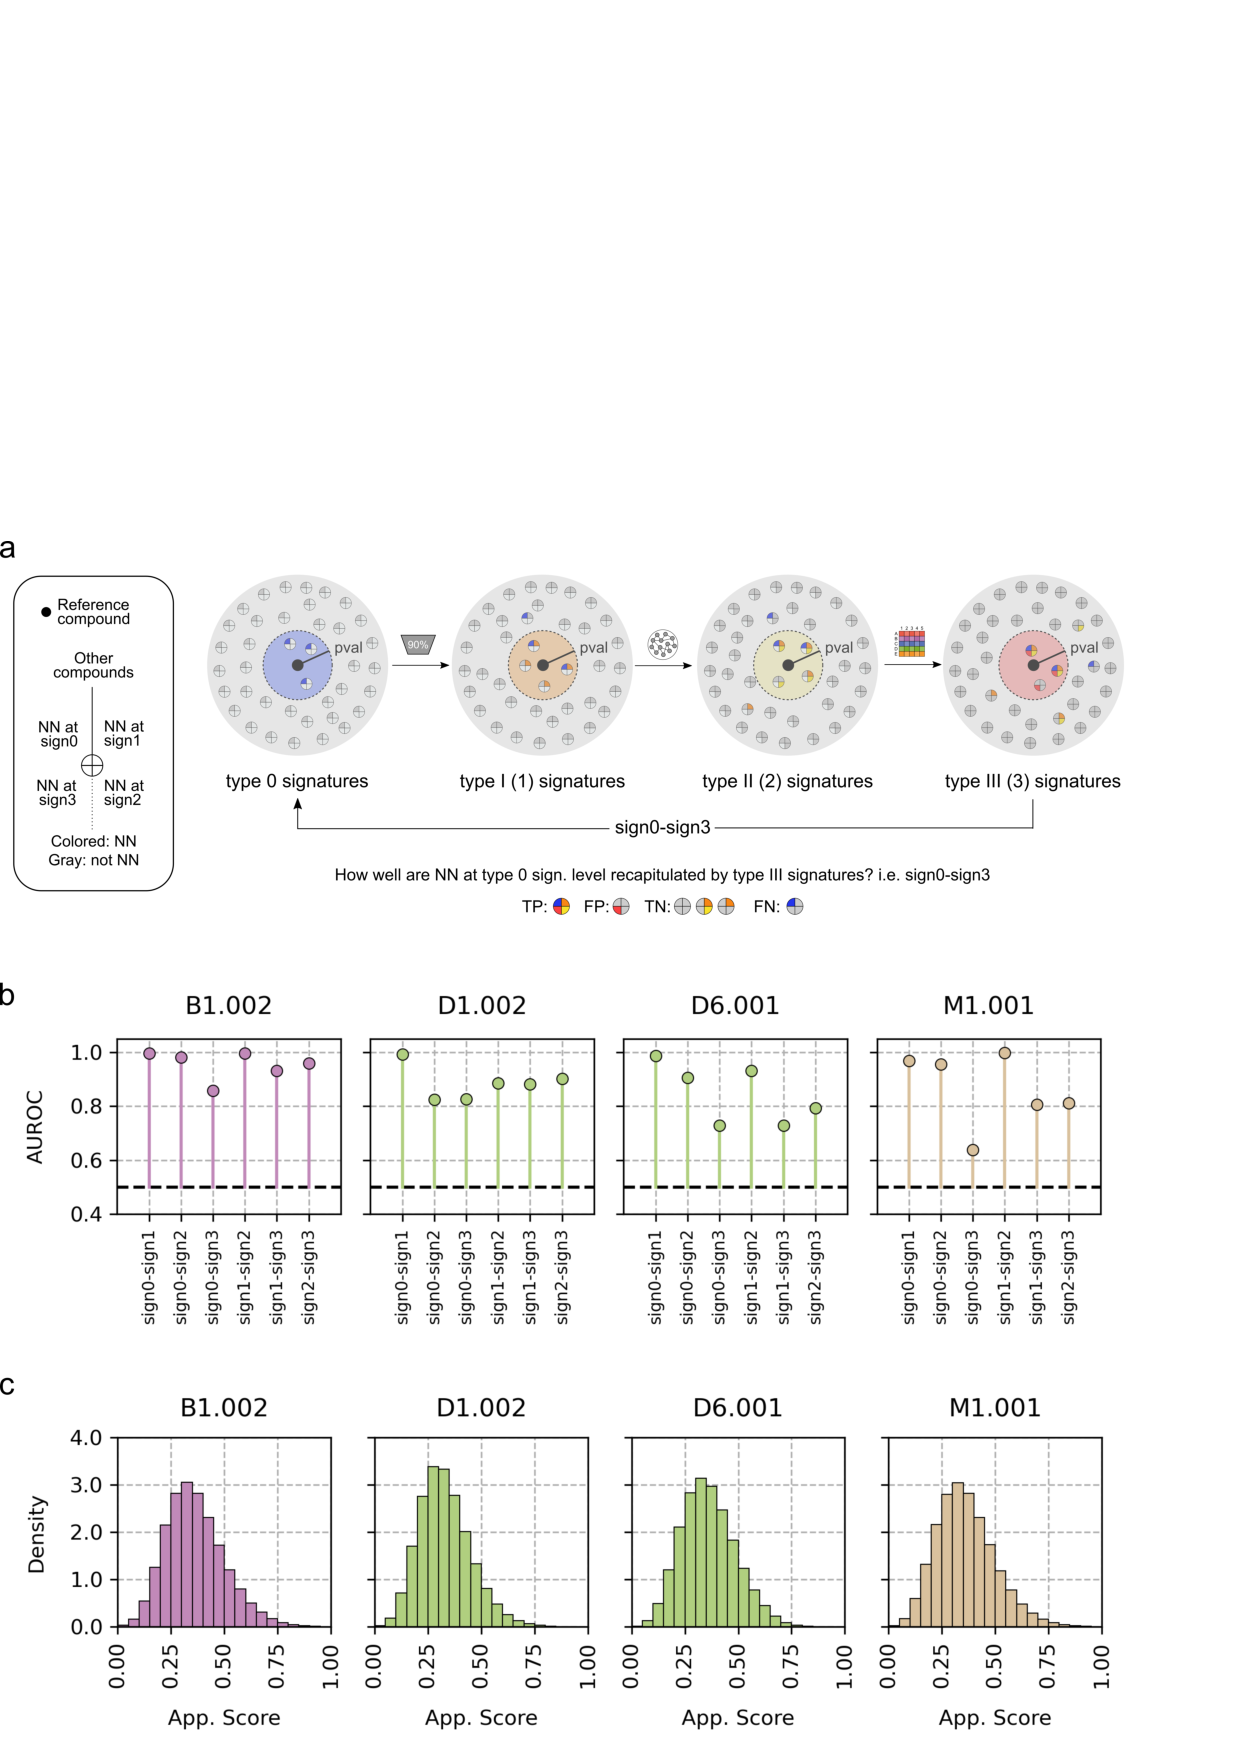
\includegraphics[width=\linewidth]{figures/PocketVec/Main/Fig3.png}
  \caption{
    \textbf{Characterization of human druggable pockets using PocketVec descriptors.} 
    \textbf{a)} Distribution of volumes (x-axis, x10³ A³) for each pocket set: PDB-LIG (1,604 pockets, red), PDB-PD (14,413 pockets, orange), AF2-LIG (1,405 pockets, purple) and AF2-PD (32,302 pockets, blue). All distributions are normalized (density, y-axis). The average volumes are 2992.88 A³, 3764.1 A³, 2940.47 A³ and 3972.66 A³, respectively. Pocket volumes were directly calculated using the rDock\cite{ruiz-carmona_rdock_2014} CAVITY functionality. 
    \textbf{b)} Correlation between average docking rankings among all pocket sets. For each pocket set, a 128-length array containing the average docking ranking for each lead-like molecule was calculated, and these arrays were compared among pocket sets by means of the Pearson’s Correlation Coefficient. All p-values (10) are <10\textsuperscript{-25}. 
    \textbf{c)} For each pocket set, proportion of PocketVec descriptors (\%, y-axis) having less than N (x-axis) outlier molecules (i.e. molecules with positive docking scores, please see \hyperref[PocketVec_Methods]{Methods}).
    \textbf{d)} Proportion of originally dissimilar pocket pairs (y-axis, distances >threshold) classified as similar (distances <threshold) due to the artificial insertion of a growing number of outlier values (x-axis) at different distance thresholds. To run the analysis, 100,000 PocketVec distances were randomly sampled (x10 times) from PDB-LIG. Solid lines represent average results and shadowed areas correspond to minimum and maximum proportions among samples. Results did not change among pocket sets (Fig \ref{PocketVec_FigS23}).
    \textbf{e)} tSNE (t-distributed Stochastic Neighbor Embedding) representation of all PocketVec descriptors within each pocket set (PDB-LIG, PDB-PD, AF2-LIG, AF2-PD). Each pocket is represented by a single point, which is colored and sized by 2D density within the pocket set. Gray dots correspond to the background space: all PocketVec descriptors are considered at once, and are also colored and sized by 2D density.
    \textbf{f)} Distributions (density, y-axis) of maximum Tanimoto Similarity among bound ligands (x-axis, bin width: 0.02) grouped by PocketVec distance ranges (0-0.10, 0.10-0.17 and 0.17-0.4). The number of pocket pairs per PocketVec distance range is specified in parenthesis.
    \textbf{g)} Distributions (density, y-axis) of PocketVec cosine distances (x-axis) grouped by the maximum Tanimoto Similarity among bound ligands (0-0.5, 0.5-0.8, 0.8-1 and 1). The number of pocket pairs per maximum Tanimoto Similarity range is specified in parenthesis.
    \textbf{h)} Distributions (density, y-axis) of PocketVec cosine distances (x-axis) grouped by the number of shared ligands between pockets (0, 1, 2 and 3 or more). The number of pocket pairs per number of shared ligands is specified in parenthesis.
  }
  \label{PocketVec_Fig3}
\end{figure}


%%%%%%%%%%%%%%%%%%%%%%%%%%%%%%%%%%%%%%%%%%%%%%%%%%%%%%%%%%%%%%%%
%%% Systematic generation of PocketVec descriptors
%%%%%%%%%%%%%%%%%%%%%%%%%%%%%%%%%%%%%%%%%%%%%%%%%%%%%%%%%%%%%%%%

\phantomsection
\subsubsection{Systematic generation of PocketVec descriptors}
\label{PocketVec_ResultsAndDiscussion_Systematic_generation_of_PocketVec_descriptors}


Once we had identified human druggable pockets with four different approaches, we systematically generated PocketVec descriptors for all of them, using the strategy described above (Fig \ref{PocketVec_Fig1}a). The high number of pockets explored enabled an exhaustive analysis of potential dependencies between the lead-like molecules used to build the descriptors and the characterization of druggable pockets. Reassuringly, we did not find any correlation between docking rankings and molecular properties of docked compounds (e.g. molecular weight or number of heavy atoms, Fig \ref{PocketVec_FigS20} and Fig \ref{PocketVec_FigS21}, respectively). On the contrary, we observed that most molecules exhibited a complete range of rankings (from 1 to 128), although the ranking distributions showed that some molecules tended to bind with good scores in many pockets while others were mostly downranked (Fig \ref{PocketVec_FigS22}). Indeed, this tendency was observed in all pocket definition strategies, and we found significant correlations between the average docking rankings for docked lead-like molecules among different pocket sets (Fig \ref{PocketVec_Fig3}b). Such correlations showed a perfect agreement between PocketVec descriptors generated through PDB and AF2 structures, but exposed slight differences between LIG and PD results (Fig \ref{PocketVec_Fig3}b, Pearson’s CC <0.88). In line with this, we found that 88.0\% and 86.8\% of the PocketVec descriptors generated for PDB-LIG and AF2-LIG, respectively, showed no lead-like molecules with positive docking scores (i.e. outlier molecules not fitting in the pocket, see \hyperref[PocketVec_Methods]{Methods}), while the fraction was considerably higher in PDB-PD and AF2-PD sets, with 97.0\% and 98.1\% of the descriptors, respectively (Fig \ref{PocketVec_Fig3}c). This result was consistent with the differences observed in pocket volumes (Fig \ref{PocketVec_Fig3}a). Reassuringly, we found that smaller pockets (<3,000ų) tended to be more prone to exhibit outlier molecules than bigger pockets (Fisher exact test, OR >70 and p-value <10\textsuperscript{-45} for all pocket sets).


To assess if outlier compounds could have a significant effect in the generation of poor PocketVec descriptors, we randomly inserted outlier values in the descriptors and computed the fraction of originally dissimilar pocket pairs (PocketVec distance >0.17) that were incorrectly labeled as similar (distance <0.17) due to an increasing number of outlier values. We observed that the insertion of up to 80 outlier molecules (out of 128) did not significantly compromise PocketVec descriptors, leading to only \textasciitilde0.039\% of false positives (Fig \ref{PocketVec_Fig3}d and Fig \ref{PocketVec_FigS23}). In front of this strong robustness of the descriptors, in further analyses, we only discarded those very few PocketVec descriptors with more than 80 outlier molecules (10, 45, 15 and 43 descriptors from the PDB-LIG, PDB-PD, AF2-LIG and AF2-PD sets, respectively). 



%%%%%%%%%%%%%%%%%%%%%%%%%%%%%%%%%%%%%%%%%%%%%%%%%%%%%%%%%%%%%%%%
%%% Influence of protein flexibility on PocketVec descriptors
%%%%%%%%%%%%%%%%%%%%%%%%%%%%%%%%%%%%%%%%%%%%%%%%%%%%%%%%%%%%%%%%

\phantomsection
\subsubsection{Influence of protein flexibility on PocketVec descriptors}
\label{PocketVec_ResultsAndDiscussion_Influence_of_protein_flexibility}

Proteins are dynamic entities that may adopt various 3D conformations depending on multiple environmental factors (e.g. the presence of a ligand), as well as exhibiting a certain degree of flexibility in their side chains. Indeed, a single X-ray structure often does not represent the complete structural behavior of a protein, and we thus do not expect a single PocketVec descriptor to be a global representation of a pocket but instead a snapshot for each particular structure. To some extent, the ProSPECCTs benchmark set already assesses the sensitivity of PocketVec descriptors to the binding site definition (i.e. same pocket occupied by distinct ligands, P1 and P1.2) and the impact of protein flexibility (i.e. NMR-resolved structures, P2). In this context, we observed that, as expected, the variability among PocketVec descriptors from the same pocket was lower enough to be clearly distinguished from random pairs of pockets (Fig \ref{PocketVec_Fig1}d, AUROCs of 0.97, 1.00 and 0.96 for ProSPECCTs P1, P1.2 and P2, respectively). Besides, a 2D tSNE representation of PocketVec descriptors derived from the 326 structures in P1 showed a clustering pattern consistent with the 12 pockets represented (Fig \ref{PocketVec_Fig4}a). Interestingly, we observed that one of the structures (3UAB\_B) of Poly-ADP polymerase tankyrase-2 (Q9H2K2) significantly deviated from the rest of the descriptors from the same pocket (protein) in the tSNE representation (black dots), and a visual inspection of its structure showed significant conformational changes in the side chains conforming the binding pocket with respect to the other ones (Fig \ref{PocketVec_Fig4}b), which translated into a higher PocketVec distance (>0.17) with the rest of the descriptors of the same pocket. In any case and, as briefly mentioned above, PocketVec descriptors for holo structures of the same pocket (ProSSPECTs P1 similar pairs) were fairly similar, with almost 80\% of the pairs showing distances <0.17, while only 1,2\% of the pairs showed distances <0.17 for dissimilar pocket pairs. When comparing holo structures to the corresponding apo structures or AF2 models of the same pocket, we found that the PocketVec descriptors showed higher variability than within \textit{holo} structures, reflecting pocket structural heterogeneity (Fig \ref{PocketVec_FigS24}). However, the distributions of distances comparing \textit{holo} with \textbf{apo} or AF2 structures were very similar, with 51\% and 55\% of pairs pairs below the 0.17 threshold, respectively. To further complement this result, we performed an exhaustive evaluation of the behavior of PocketVec descriptors upon protein flexibility and conformational changes. In short, we kept those pockets from the PDB-LIG set for which we had enough \textit{holo} and \textit{apo} PDB structures available (≥10, see \hyperref[PocketVec_Methods]{Methods}) as well as a confident AF2 model, and generated PocketVec descriptors for all their structures. Overall, we collected 903 PocketVec descriptors corresponding to 43 unique pockets (10 holo structures, 10 apo structures and 1 AF2 model each). We then computed PocketVec distances between same-pocket holo PDB structures (LIG-LIG), same-pocket holo and apo PDB structures (LIG-PD), same-pocket apo PDB structures (PD-PD), same-pocket holo PDB and AF2 structures (LIG-AF2) and, finally, same-pocket apo PDB and AF2 structures (PD-AF2). Additionally, we compared holo (PDB), apo (PDB) and AF2 structures against our 4 sets of precompiled PocketVec descriptors (i.e. PDB-LIG, PDB-PD, AF2-LIG and AF2-PD) in order to contextualize the results with background distance distributions (Fig \ref{PocketVec_Fig4}c). We observed that PocketVec descriptors derived from holo PDB structures were rather robust and clearly distinguishable from random pocket pairs (LIG-LIG, AUROC of 0.90 against background distance distributions), in perfect agreement with the results obtained in ProSPECCTs P1 and P1.2. When we compared descriptors derived from holo and apo PDB structures, as expected, the intrinsic and increased variability of ligand-free structures was reflected in the PocketVec distances, which affected the ability to recapitulate pocket structures from the same protein (LIG-PD, AUROC of 0.77; PD-PD, AUROC of 0.80). Finally, we also observed that descriptors derived from holo structures tended to be more similar to those derived from AF2 models than to those from apo PDB structures (LIG-AF2, AUROC of 0.82). This observation aligns with several studies stating that AF2-predicted structures are comparable to the apo conformations and, perhaps, a bit closer to the holo conformations due to the nature of the training data (which includes both holo and apo structures)\cite{zhang_benchmarking_2023}.


Additionally, we sampled MD trajectories for 192 pockets from the PDB-LIG and PDB-PD sets, considering 10 conformations per pocket, and then, for each pocket, we calculated all pairwise distances among their PocketVec descriptors (see Online Methods). As in the previous exercise, we also compared the obtained PocketVec descriptors with a random sample of precomputed descriptors from the PDB-LIG, PDB-PD, AF2-LIG and AF2-PD sets (Fig \ref{PocketVec_Fig4}d). Overall, we observed a similar trend than when comparing \textit{apo} PDB structures: PocketVec descriptors showed variations responding to the flexibility of the proteins, while still recognizing different conformations from the same pocket (AUROC of 0.78). Finally, we analyzed the correlation between PocketVec distance among MD frames and the all-atom RMSD (excluding hydrogen atoms) considering both complete structures and only pocket residues (at <8Å from the pocket centroid in any of the MD used frames). We found a weak correlation (Fig \ref{PocketVec_Fig4}e; Pearson CC 0.39) with the full structure RMSD that increased (Fig \ref{PocketVec_Fig4}f; Pearson CC 0.49) when exclusively considering pocket residues. 

The presence of metal atoms is often required for many pockets to perform its native function (e.g. to act as catalytic centers or to stabilize protein structures). However, our study does not explicitly consider the presence of other compounds such as cofactors or metal atoms which, despite the limitations, it enables a fair and analogous characterization with different protein structures and pocket identification strategies where bound metal atoms are not available (e.g. PDB vs AF2 or LIG vs PD). Thus, finally, we also assessed the ability of our precomputed PocketVec descriptors to identify pocket similarities among metal-binding proteins. For this, after collecting all PDB-LIG and PDB-PD pockets with bound metal atoms, we compared the derived PocketVec descriptors with and without the metal atoms (\hyperref[PocketVec_Methods]{Methods}). We observed that, although descriptors were obviously not identical, the vast majority of the identified metal-binding pockets had similar PocketVec descriptors with and without the explicit presence of the metal atoms (Mann-Whitney p-value <10\textsuperscript{-100}; Fig \ref{PocketVec_FigS25}). 

Overall, these results illustrate the capacity of PocketVec descriptors to capture pocket flexibility and protein conformational changes, revealing their sensitivity to changes in the pocket shapes as well as their feasibility of use with \textit{holo} and \textit{apo} PDB structures (including metal-binding proteins) and AF2 predicted models. 










%%%%%%%%%%%%%%%%%%%%%%%%%%%%%%%%%%%%%%%%%%%%%%%%%%%%%%%%%%%%%%%%
%%% All-vs-all comparison of human druggable pockets
%%%%%%%%%%%%%%%%%%%%%%%%%%%%%%%%%%%%%%%%%%%%%%%%%%%%%%%%%%%%%%%%

\phantomsection
\subsubsection{All-vs-all comparison of human druggable pockets}
\label{PocketVec_ResultsAndDiscussion_All_vs_All_comparison_human_druggable_pockets}


Bla bla bla







%%%%%%%%%%%%%%%%%%%%%%%%%%%%%%%%%%%%%%%%%%%%%%%%%%%%%%%%%%%%%%%%
%%% Relationship between PocketVec similarity and experimentally determined compound-target pairs
%%%%%%%%%%%%%%%%%%%%%%%%%%%%%%%%%%%%%%%%%%%%%%%%%%%%%%%%%%%%%%%%

\phantomsection
\subsubsection{Relationship between PocketVec similarity and experimentally determined compound-target pairs}
\label{PocketVec_ResultsAndDiscussion_Relationship_PocketVecSimilarity_CPD-TARGET_pairs}


Bla bla bla









%%%%%%%%%%%%%%%%%%%%%%%%%%%%%%%%%%%%%%%%%%%%%%%%%%%%%%%%%%%%%%%%
%%% Identifying kinases with similar inhibition profiles through PocketVec descriptors
%%%%%%%%%%%%%%%%%%%%%%%%%%%%%%%%%%%%%%%%%%%%%%%%%%%%%%%%%%%%%%%%

\phantomsection
\subsubsection{Identifying kinases with similar inhibition profiles through PocketVec descriptors}
\label{PocketVec_ResultsAndDiscussion_Identifying_Kinases}


Bla bla bla


